%%%%%%%%%%%%%%%%%%%%%%%%%%%%%%%%%%%%%%%%%
% Beamer Presentation
% LaTeX Template
% Version 1.0 (10/11/12)
%
% This template has been downloaded from:
% http://www.LaTeXTemplates.com
%
% License:
% CC BY-NC-SA 3.0 (http://creativecommons.org/licenses/by-nc-sa/3.0/)
%
%%%%%%%%%%%%%%%%%%%%%%%%%%%%%%%%%%%%%%%%%

%----------------------------------------------------------------------------------------
%	PACKAGES AND THEMES
%----------------------------------------------------------------------------------------

\documentclass[hideothersubsections, t, aspectratio=1610]{beamer}

\mode<presentation> {

% The Beamer class comes with a number of default slide themes
% which change the colors and layouts of slides. Below this is a list
% of all the themes, uncomment each in turn to see what they look like.

%\usetheme{default}
%\usetheme{AnnArbor}
%\usetheme{Antibes}
%\usetheme{Bergen}
%\usetheme{Berkeley}
%\usetheme{Berlin}
%\usetheme{Boadilla}
%\usetheme{CambridgeUS}
%\usetheme{Copenhagen}
%\usetheme{Darmstadt}
%\usetheme{Dresden}
%\usetheme{Frankfurt}
%\usetheme{Goettingen}
%\usetheme{Hannover}
%\usetheme{Ilmenau}
%\usetheme{JuanLesPins}
%\usetheme{Luebeck}
%\usetheme{Madrid}
%\usetheme{Malmoe}
%\usetheme{Marburg}
%\usetheme{Montpellier}
\usetheme{PaloAlto}
%\usetheme{Pittsburgh}
%\usetheme{Rochester}
%\usetheme{Singapore}
%\usetheme{Szeged}
%\usetheme{Warsaw}

% As well as themes, the Beamer class has a number of color themes
% for any slide theme. Uncomment each of these in turn to see how it
% changes the colors of your current slide theme.

%\usecolortheme{albatross}
%\usecolortheme{beaver}
%\usecolortheme{beetle}
%\usecolortheme{crane}
%\usecolortheme{dolphin}
%\usecolortheme{dove}
%\usecolortheme{fly}
%\usecolortheme{lily}
\usecolortheme{orchid}
%\usecolortheme{rose}
%\usecolortheme{seagull}
%\usecolortheme{seahorse}
%\usecolortheme{whale}
%\usecolortheme{wolverine}

%\setbeamertemplate{footline} % To remove the footer line in all slides uncomment this line
%\setbeamertemplate{footline}[page number] % To replace the footer line in all slides with a simple slide count uncomment this line

%\setbeamertemplate{navigation symbols}{} % To remove the navigation symbols from the bottom of all slides uncomment this line
}

\usepackage{graphicx} % Allows including images
\usepackage{booktabs} % Allows the use of \toprule, \midrule and \bottomrule in tables
\usepackage{tikz}
\usepackage{comment}
\usepackage{minted}
%---------------------------------------------------------------------------------------------
%%  This file is really -*-LaTeX-*-
%%             File:  thesis-macros.sty
%%          Created:  Sat Feb 20 23:33:41 2016
%%
%%      Description:  Commands particular to this thesis

\newsavebox\xXx
\newcommand{\xxx}[1]{\savebox\xXx{#1}#1\kern-1.0\wd\xXx\textcolor{red}{\rule[0.7ex]{\wd\xXx}{1pt}}%
	\kern-1.0\wd\xXx\textcolor{red}{\rule[0.25ex]{\wd\xXx}{1pt}}%
}
\newcommand{\replace}[2]{\xxx{#1}\,{\color{blue}#2}}
\let\yyy\replace

\newcommand{\progLang}[1]{\textsc{#1}}
\newcommand{\unknownLabel}[1]{\texttt{\large\color{dark-red}\slshape #1}}
\newcommand{\markWord}[1]{\unknownLabel{#1}\eref{text-kind}}
\newcommand{\chapterReference}[2]{\textcolor{blue}{\underline{\hyperref[#1]{#2}}}}

\definecolor{dark-purple}{rgb}{0.40,0.05,0.40}\relax
\definecolor{dark-red}{rgb}{0.50,0.00,0.00}\relax
\definecolor{dark-green}{rgb}{0.00,0.50,0.00}\relax
\definecolor{fuchsia}{rgb}{0.99,0.50,0.99}\relax
\newcommand*{\mehul}[1]{\textcolor{dark-red}{#1}}
\newcommand*{\david}[1]{\textcolor{dark-green}{#1}}
\newcommand\firstOfTwo[2]{#1}
\newcommand\secondOfTwo[2]{#2}
\newcommand{\enparen}[1]{\textup{\firstOfTwo()}#1\textup{\secondOfTwo()}}
\newcommand{\macroName}[1]{\texttt{\char`\\#1}}
\newcommand{\macroArg}[1]{\texttt{\char`\{#1\char`\}}}
\newcommand{\prologConstruct}[1]{\textcolor{brown}{\texttt{#1}}}
\newcommand{\haskellConstruct}[1]{\textcolor{magenta}{\texttt{#1}}}
\newcommand{\haskellClass}[1]{\haskellConstruct{#1}}
\newcommand{\haskellVar}[1]{\haskellConstruct{\textit{#1}}}
\newcommand{\languageConstruct}[1]{\textcolor{orange}{\texttt{#1}}}
\newcounter{butCounter}
\newcommand\butbut{\addtocounter{butCounter}{1}\edef\next{%
		\noexpand\endnote{This is sentence \# \arabic{butCounter} starting %
			with ``But''.}}\next}

\providecommand\codeLibrary[1]{\texttt{\bfseries #1}}
\providecommand\metaSyntacticVariable[1]{\textsl{\ttfamily #1}}
\providecommand\mSV{\metaSyntacticVariable}

%----------------------------------------------------------------------------------------
%	TITLE PAGE
%----------------------------------------------------------------------------------------
\title[]{Embedding  Programming Languages: \newline \progLang{Prolog} in \progLang{Haskell}} % The short title appears at the bottom of every slide, the full title is only on the title page

\author{Mehul Solanki} % Your name
\institute[UNBC] % Your institution as it will appear on the bottom of every slide, may be shorthand to save space
{
	University of Northern British Columbia \newline \\ % Your institution for the title page
	\medskip
	\textit{solanki@unbc.ca} % Your email address
}
\date{\today} % Date, can be changed to a custom date

\begin{document}
	\setbeamertemplate{footline}[frame number]
	\setbeamertemplate{itemize items}[circle]
	\setbeameroption{show notes} % un-comment to see the notes
	\begin{frame}
		\titlepage % Print the title page as the first slide
		\note[item]{Good afternoon everybody. My name is Mehul Solanki. I am a graduate student in the computer science department 
		under  Dr. David Casperson. And today I would like to talk about embedding \progLang{Prolog} in \progLang{Haskell}.}
	\end{frame}

%% ====================================================================-
%% ====================================================================-
\section{Introduction}


%% -------------------------------------------------------------------
\begin{frame}[allowframebreaks=1.1]
\frametitle{Introduction} % Table of contents slide, comment this block out to remove it
\tableofcontents % Throughout your presentation, if you choose to use \section{} and \subsection{} commands, these will automatically be printed on this slide as an overview of your presentation
\note[item]{We will begin with languages and how they are combined.}
\note[item]{The problem this thesis contributes to.}
\note[item]{Some concepts and the prototype implementations.}
\note[item]{And lastly, we sum up with possible directions.} 
\note[item]{So let's get started.}
\end{frame}
%% -------------------------------------------------------------------




%% ====================================================================-
%% ====================================================================-
\section{Background}

%% -------------------------------------------------------------------
\begin{frame}{Background Overview}
\frametitle{Background Overview}

\begin{itemize}
\note[item]{In this section we will talk about,}
\item Programming languages and \progLang{Haskell} and \progLang{Prolog}.
\note[item]{Programming languages and programming paradigms.}
\note[item]{along with the languages in question, \progLang{Haskell} and \progLang{Prolog},}

\item Classification.
\note[item]{How they are classified}

\item Programming paradigms and declarative programming.
\note[item]{Next paradigms and the declarative stlye of programming in particular,} 

\item Functional and logic programming.
\note[item]{and it's sub-paradigms functional and logic programming,}

\item Bringing programming languages together.
\note[item]{lastly the approaches for bringing programming languages together.}
\end{itemize}
\end{frame}
%% -------------------------------------------------------------------

%% ====================================================================-
\subsection{Programming Languages}
\begin{frame}{Programming Languages}
\begin{columns}[T]
    \begin{column}{.4\textwidth}
     \begin{block}{}
A programming language is an artificial language designed to communicate instructions to a machine, particularly a computer.
\\*For example, \textsc{C, Java}.
    \end{block}
    \end{column}
    \begin{column}{.6\textwidth}
    \begin{block}{}
% Your image included here
\begin{figure}[H]
    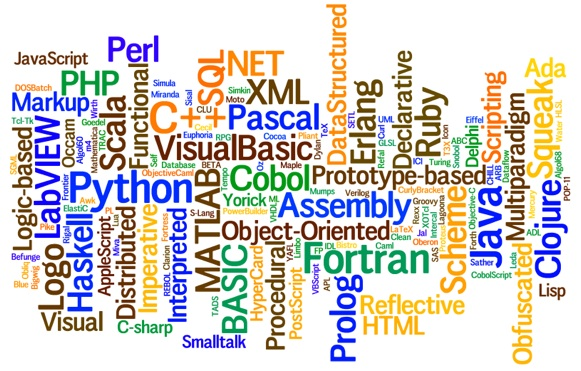
\includegraphics[width=1\textwidth]{progLanguages.jpg}
    
    \caption{The Universe of Programming Languages}
 \end{figure}   
    \end{block}
    \end{column}
  \end{columns}
\note[item]{A programming language is used to communicate instructions to a computer.}
\note[item]{They are in the hundereds of thousands and the number keeps on increasing.}
\end{frame}

%% -------------------------------------------------------------------
\begin{frame}
\frametitle{\progLang{Haskell}}
 \note[item]{So \progLang{Haskell} is a functional language,} 
  \begin{columns}[T]
    \begin{column}{.7\textwidth}
     \begin{block}{}
\progLang{Haskell} is an advanced purely-functional programming language. In particular, it is a 
\begin{itemize}
\item Polymorphically statically typed,
\note[item]{which is statically typed meaning every expression in Haskell has a type which is determined at compile time.}

\item Type inference,
\note[item]{has type type inference meaning you don't have to explicitly write out every type in a Haskell program.}

\item Lazy,
\note[item]{is lazy meaning functions don't evaluate their arguments until required.}

\item Purely Functional.
\note[item]{and is purely funcitonal meaning every function in Haskell is a function in the mathematical sense (i.e., "pure").}
\end{itemize}

    \end{block}
    \end{column}
    \begin{column}{.3\textwidth}
    \begin{block}{}
% Your image included here
\begin{figure}
    
\includegraphics[width=\textwidth]{haskelllogo.jpg} 
    \caption{\progLang{Haskell} Programming Language}
 \end{figure}   
    \end{block}
    \end{column}
  \end{columns}
\end{frame}
%% -------------------------------------------------------------------




\begin{comment}
%% ====================================================================-
\subsection{Logic Programming}
%% -------------------------------------------------------------------
\begin{frame}{Logic Programming}
\begin{itemize}
\item Logic programming.
\note[item]{is based on formal logic. A program consists of a set of rules used to derive a solution.}

\item Universal Horn clauses.
\note[item]{A Horn clause is a clause (a disjunction of literals) with at most one positive literal.}

\item For example, \progLang{Prolog}.
\end{itemize}
\end{frame}
%% -------------------------------------------------------------------

\end{comment}

%% -------------------------------------------------------------------
\begin{frame}
\frametitle{\progLang{Prolog}}
  \begin{columns}[T]
    \begin{column}{.6\textwidth}
     \begin{block}{}
General purpose logic programming language with over 20 distributions. \progLang{Prolog} is a programming language borrowing its basic 
constructs from logic. A pure \progLang{Prolog} program is a logic program, in which an order is defined for both clauses in the program and 
for goals in the body of the clause.
\note[item]{\progLang{Prolog} is a general purpose programming language in which programs consist of facts and rules used to solve a 
query.}
\note[item]{It has a number of distributions, \progLang{SWI Prolog} being one of the popular ones.}
    \end{block}
    \end{column}
    \begin{column}{.4\textwidth}
    \begin{block}{}
% Your image included here
\begin{figure}
    
\includegraphics[width=\textwidth]{swipl.png} 
    \caption{\textsc{SWI Prolog} Distribution}
 \end{figure}   
    \end{block}
    \end{column}
  \end{columns}
\end{frame}
%% -------------------------------------------------------------------

%% ====================================================================-
\subsection{Programming Language Paradigms}
\begin{frame}
\frametitle{Programming Language Paradigms}
  \begin{columns}[T]
    \begin{column}{.4\textwidth}
     \begin{block}{}
A programming paradigm is a fundamental style of computer programming, a way of building the structure and elements of computer programs.
\\*For example, Object Oriented Programming.
    \end{block}
    \end{column}
    \begin{column}{.6\textwidth}
    \begin{block}{}
% Your image included here
\begin{figure}
    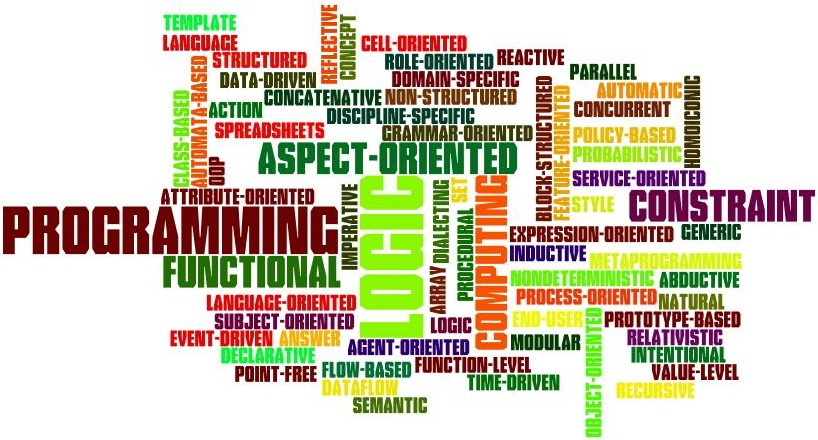
\includegraphics[width=1\textwidth]{programminglanguageparadigms.jpg} 
    \caption{Programming Paradigms}
 \end{figure}   
    \end{block}
    \end{column}
  \end{columns}
  \note[item]{The fundamental style or manner in which a computer program is built is known as a programming paradigm.}
  \note[item]{For example, the object oriented style of programming.}
\end{frame}

\begin{frame}
\frametitle{Classification}
  \begin{columns}[T]
    \begin{column}{.5\textwidth}
     \begin{block}{}
Programming languages are classified into paradigms depending on their characteristics and features. 
\\*For example, \progLang{Java} is an Object Oriented Programming Language.
    \end{block}
    \end{column}
    \begin{column}{.5\textwidth}
    \begin{block}{}
% Your image included here
\begin{figure}
    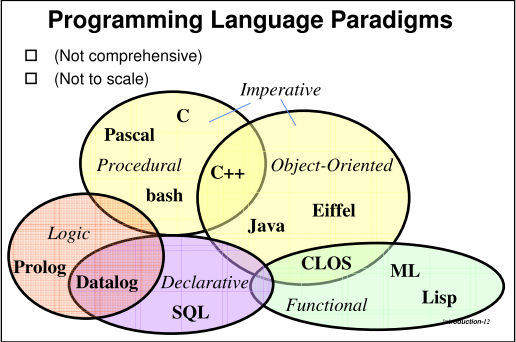
\includegraphics[width=\textwidth]{classification.png} 
    \caption{Classification of Programming Languages}
 \end{figure}   
    \end{block}
    \end{column}
  \end{columns}
  \note[item]{Depending on the characteristics exhibited by a language into paradigms.}
  \note[item]{\progLang{Java} is an object oriented programming language.}
\end{frame}



%% -------------------------------------------------------------------
\begin{frame}
\frametitle{Declarative Programming}
\begin{itemize}
\item Declarative style of programming, describe (declaratively) what to do and not (operationally) how to do it. 
\note[item]{http://www.eolss.net/sample-chapters/c15/e6-45-05-04.pdf}
\note[item]{One such style is the declarative paradigm, where we describe the logic of a computation without the control flow.[Practical 
Advantages of Declarative Programming Lloyd, J.W]}

\note[item]{It further branches out into functional and logic programming.}

\item Programming in a functional language consists of building definitions and using the computer to evaluate expressions.
\note[item]{A funcitonal language is all about building and applying functions.}

\item In logic programming, a program consists of a collection of statements ex-pressed as formulas in symbolic logic. There are rules of 
inference from logic that allow a new formula to be derived from old ones, with the guarantee that if the old formulas are true, so is the 
new one.
\note[item]{Logic programming allows a new formula to be derived from the old ones. A logic programming consists of a set of facts and 
rules. And these are used to solve a query.}

\item For example, \progLang{Haskell}(functional language) and \progLang{Prolog}(logic language).
\note[item]{\progLang{Haskell} is a functional programming language while \progLang{Prolog} is a logic programming language.}
\note[item]{Both of them are declarative in nature but work differently.}

\end{itemize}
\end{frame}
%% -------------------------------------------------------------------

\begin{comment}
\begin{frame}
\frametitle{Functional Programming}
  \begin{columns}[T]
    \begin{column}{.6\textwidth}
     \begin{block}{}
Programming in a functional language consists of building definitions and using the computer to evaluate expressions. 
\\*For example, \progLang{Haskell}.
\note[item]{}
    \end{block}
    \end{column}
    \begin{column}{.4\textwidth}
    \begin{block}{}
% Your image included here
\begin{figure}
    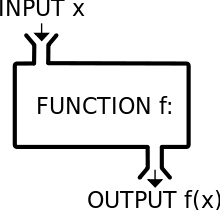
\includegraphics[width=\textwidth]{function-machine.jpeg} 
    \caption{Function}
 \end{figure}   
    \end{block}
    \end{column}
  \end{columns}
\end{frame}
\end{comment}

%% -------------------------------------------------------------------
\begin{frame}[fragile]{Functional Programming}
\note[item]{A few more details on functional programming,}
\begin{itemize}
\item $\lambda$-calculi, is a formal system in mathematical logic for expressing computations.
\note[item]{Fucntional programming works by applying mathematical functions to arguments to get results. A program is nothing but 
functions which can also be passed to other functions as arguments.}

\note[item]{The typed variant of $\lambda$-calculi puts restrictions on the type of data a function can work with.}

\item Damas-Hindley-Milner type system provides the ability to give a most general type to a function or program.
\note[item]{It is based on the Damas-Hindley-Milner type system which provides the most general type to a function or program.}
\begin{minted}[linenos]{haskell}
add :: Int -> Int -> Int
add x y = x + y
\end{minted}

\note[item]{For example, the \haskellConstruct{add} function takes as input two integers and returns their sum as the result.}

\item For example, \progLang{Scheme} and \progLang{Lisp}.

\item Side-effect free.
\note[item]{Functional programs are side-effect free, meaning, the state is not modified in any way when the functions are executed.}
\note[item]{Our \haskellConstruct{add} function does not change the values of x or y and just returns their sum.}
\end{itemize}
\end{frame}
%% -------------------------------------------------------------------





%% ====================================================================-
\subsection{Combining Programming Languages}

%% -------------------------------------------------------------------
\begin{frame}
\frametitle{Embedding Languages}
\note[item]{This section deals with embedding a target language in to the host environement.}
\note[item]{The aim of this approach is to bring the target language functionalities to the host language.}

Implementing a language within another language.

\begin{itemize}
\item Foreign Function Interface (FFI)
 \\* A mechanism by which a program written in one programming language can make use of services written in another language. 
\\* For example, \progLang{Haskell} provides a mechanism to embed \progLang{C} code in its programs.
\note{A foreign function interface allows programs to cooperate with programs written with other languages.}

\item Library or Module Extension
\\* Replicate the features and characteristics of the target language into the host. 
\\* For example, \progLang{LogLisp} is \progLang{Prolog} library for \progLang{Lisp}. 
\note[item]{A micro language is implemented using the host language constructs to replicate the target language.}
\end{itemize}

\end{frame}
%% -------------------------------------------------------------------

%% -------------------------------------------------------------------
\begin{frame}{Embedding \progLang{Prolog}}
\note[item]{This section deals with embedding a target language in the host environement.}
\note[item]{The aim of this approach to bring the target language functionalities to the host language.}
\begin{itemize}
\item Embedding \progLang{Prolog}.
\note[item]{\progLang{Prolog} is a very popular choice as a target language.}

\item Host languages : \progLang{Java, Lisp, Scheme}.
\note[item]{Implementations exist for languages like \progLang{Java, Lisp} and \progLang{Scheme}.}

\item \progLang{Prolog} in \progLang{Haskell} : 
\note[item]{A few \progLang{Prolog} implementations do exist for \progLang{Haskell}.}
\begin{itemize}
\item \codeLibrary{Mini Prolog} : A micro \progLang{Prolog}-like language for an older specification for \progLang{Haskell} 98.

\item \codeLibrary{prolog} : A \progLang{Prolog}-like interpreter which can be interacted through a REPL.
\end{itemize}
 \note[item]{None of these are currently under active development and provide limited funcitonality. }
 \note[item]{Though we use components from these implementations, they do not utilize the haskellian features that makes life a lot simpler as we shall see.}

\item Logic programming in \progLang{Haskell}.
\note[item]{For adding logic programming capabiliies to \progLang{Haskell} there exist,}
\begin{itemize}
\item Propositional logic,
\item Backtracking, and,
\item Unification.
\end{itemize}
\note[item]{libraries related to propositional logic, backtracking and unification.}
\end{itemize}
\end{frame}
%% -------------------------------------------------------------------




%% -------------------------------------------------------------------
\begin{frame}
\note[item]{In this section we talk about languages that exhibit properties from multiple paradigms.}
\frametitle{Merging Paradigms}
\begin{itemize}
\item Combining different programming paradigms or programming styles into a single environment resulting in a hybrid language.
\note[item]{Attemp to combine properties(many a times conflicting in nature) of languages and/or paradigms }

\item The idea of a multi paradigm language is to provide a framework in which programmers can work in a variety of styles, freely
intermixing constructs from different paradigms.
\note[item]{A multi-paradigm programming language is a programming language that supports more than one programming paradigm allowing the 
	programmer to work in a variety of styles.[https://developer.mozilla.org/ar/docs/multiparadigmlanguage.html]}

\item For example, \progLang{Scala} is an object functional programming language.
\note[item]{A notable example is \progLang{Scala}, object functional language based on \progLang{Java}. Simply put it is Java with strong 
	funcitonal characteristics such as higher order functions.}

\item Functional Logic programming languages.
\note[item]{are hybrid declarative languages exhibiting functional and logic programming languages.}

\item For example, \progLang{Curry}.
\note[item]{is a \progLang{Haskell} based functional logic programming language providing the choice operator for non deterministic
	operations along with two way pattern matching.}

\item Other examples, \progLang{Mercury}.
\note[item]{which goes the other way round, starting from \progLang{Prolog} and adding \progLang{Haskell} features.}

\end{itemize}

\end{frame}
%% -------------------------------------------------------------------


%% ====================================================================-
%% ====================================================================-
\section{The Problem}

%% ====================================================================-
\subsection{Language Selection}
%% -------------------------------------------------------------------
\begin{frame}
	\frametitle{Choosing a Language}
	\note[item]{The versatility of a programming language is how well it can adapt to a particular problem.}

 \begin{columns}[T]
  \begin{column}{0.5\textwidth}
   \begin{block}{General Purpose Language}
    \textcolor{dark-green}{Broad scope} but \textcolor{red}{problem needs to be moulded according to the capability of the language}.
    \note[item]{A truly general purpose programming language, GPL, is described which contains facilities for constructing (within the 
     language) new data types as well as facilities for operations performed upon them.[Jan V. Garwick. 1968. Programming Languages: GPL, a 
     truly general purpose language. Commun. ACM 11, 9 (September 1968), 634-638. DOI=http://dx.doi.org/10.1145/364063.364092]}
   \end{block}
  \end{column}

  \begin{column}{0.5\textwidth}
   \begin{block}{Special Purpose Language}
    \textcolor{red}{Limited scope} but \textcolor{dark-green}{easier to express the problem as the suitable capabilities are readily available}. 
 	 \note[item]{A domain specific language is a concise micro language that offers tools and functionalities focused on solving problems 
 	 in a particular domain.} 
   \end{block}
  \end{column}
 \end{columns}

\begin{itemize}
\item For example, "Clarissa", a voice user interface for browsing procedures on the International Space Station.
	\note[item]{For instance, \progLang{Prolog} is good for rule based systems. "Clarissa", a voice user interface for browsing space station procedures is written in SICStus
		Prolog[https://ti.arc.nasa.gov/m/pub-archive/999h/0999\%20\%28Rayner\%29.pdf].}
	\note[item]{Simply speaking, it is like "siri" for the International Space Station.}
\end{itemize}
 
\end{frame}
%% -------------------------------------------------------------------

\begin{comment}
	%% ====================================================================-
\subsection{Languages}
\begin{frame}{Languages}
\begin{itemize}
\item Selection
\note[item]{Choosing a language is quite a daunting task. There are costs related to migration, training among others.}

\item Replicating functionality.
\note[item]{One option is to replicate the target language funcitonality in the current environment, and that is what we will look at 
today. Replicating \progLang{Prolog}-like functionality in \progLang{Haskell}}
\note[item]{The result is something close to a \textit{haskellised} \progLang{Prolog}, a functional eDSl with logic programming 
capabilities.}

\end{itemize}

\end{frame}
\end{comment}

%% ====================================================================-
\begin{frame}
\frametitle{Programmer's Dilemma}
\note[item]{Choosing a language is quite a daunting task. There are costs related to migration, training among others.}
\note[item]{And not to mention the plethora of options.}
\begin{figure}
    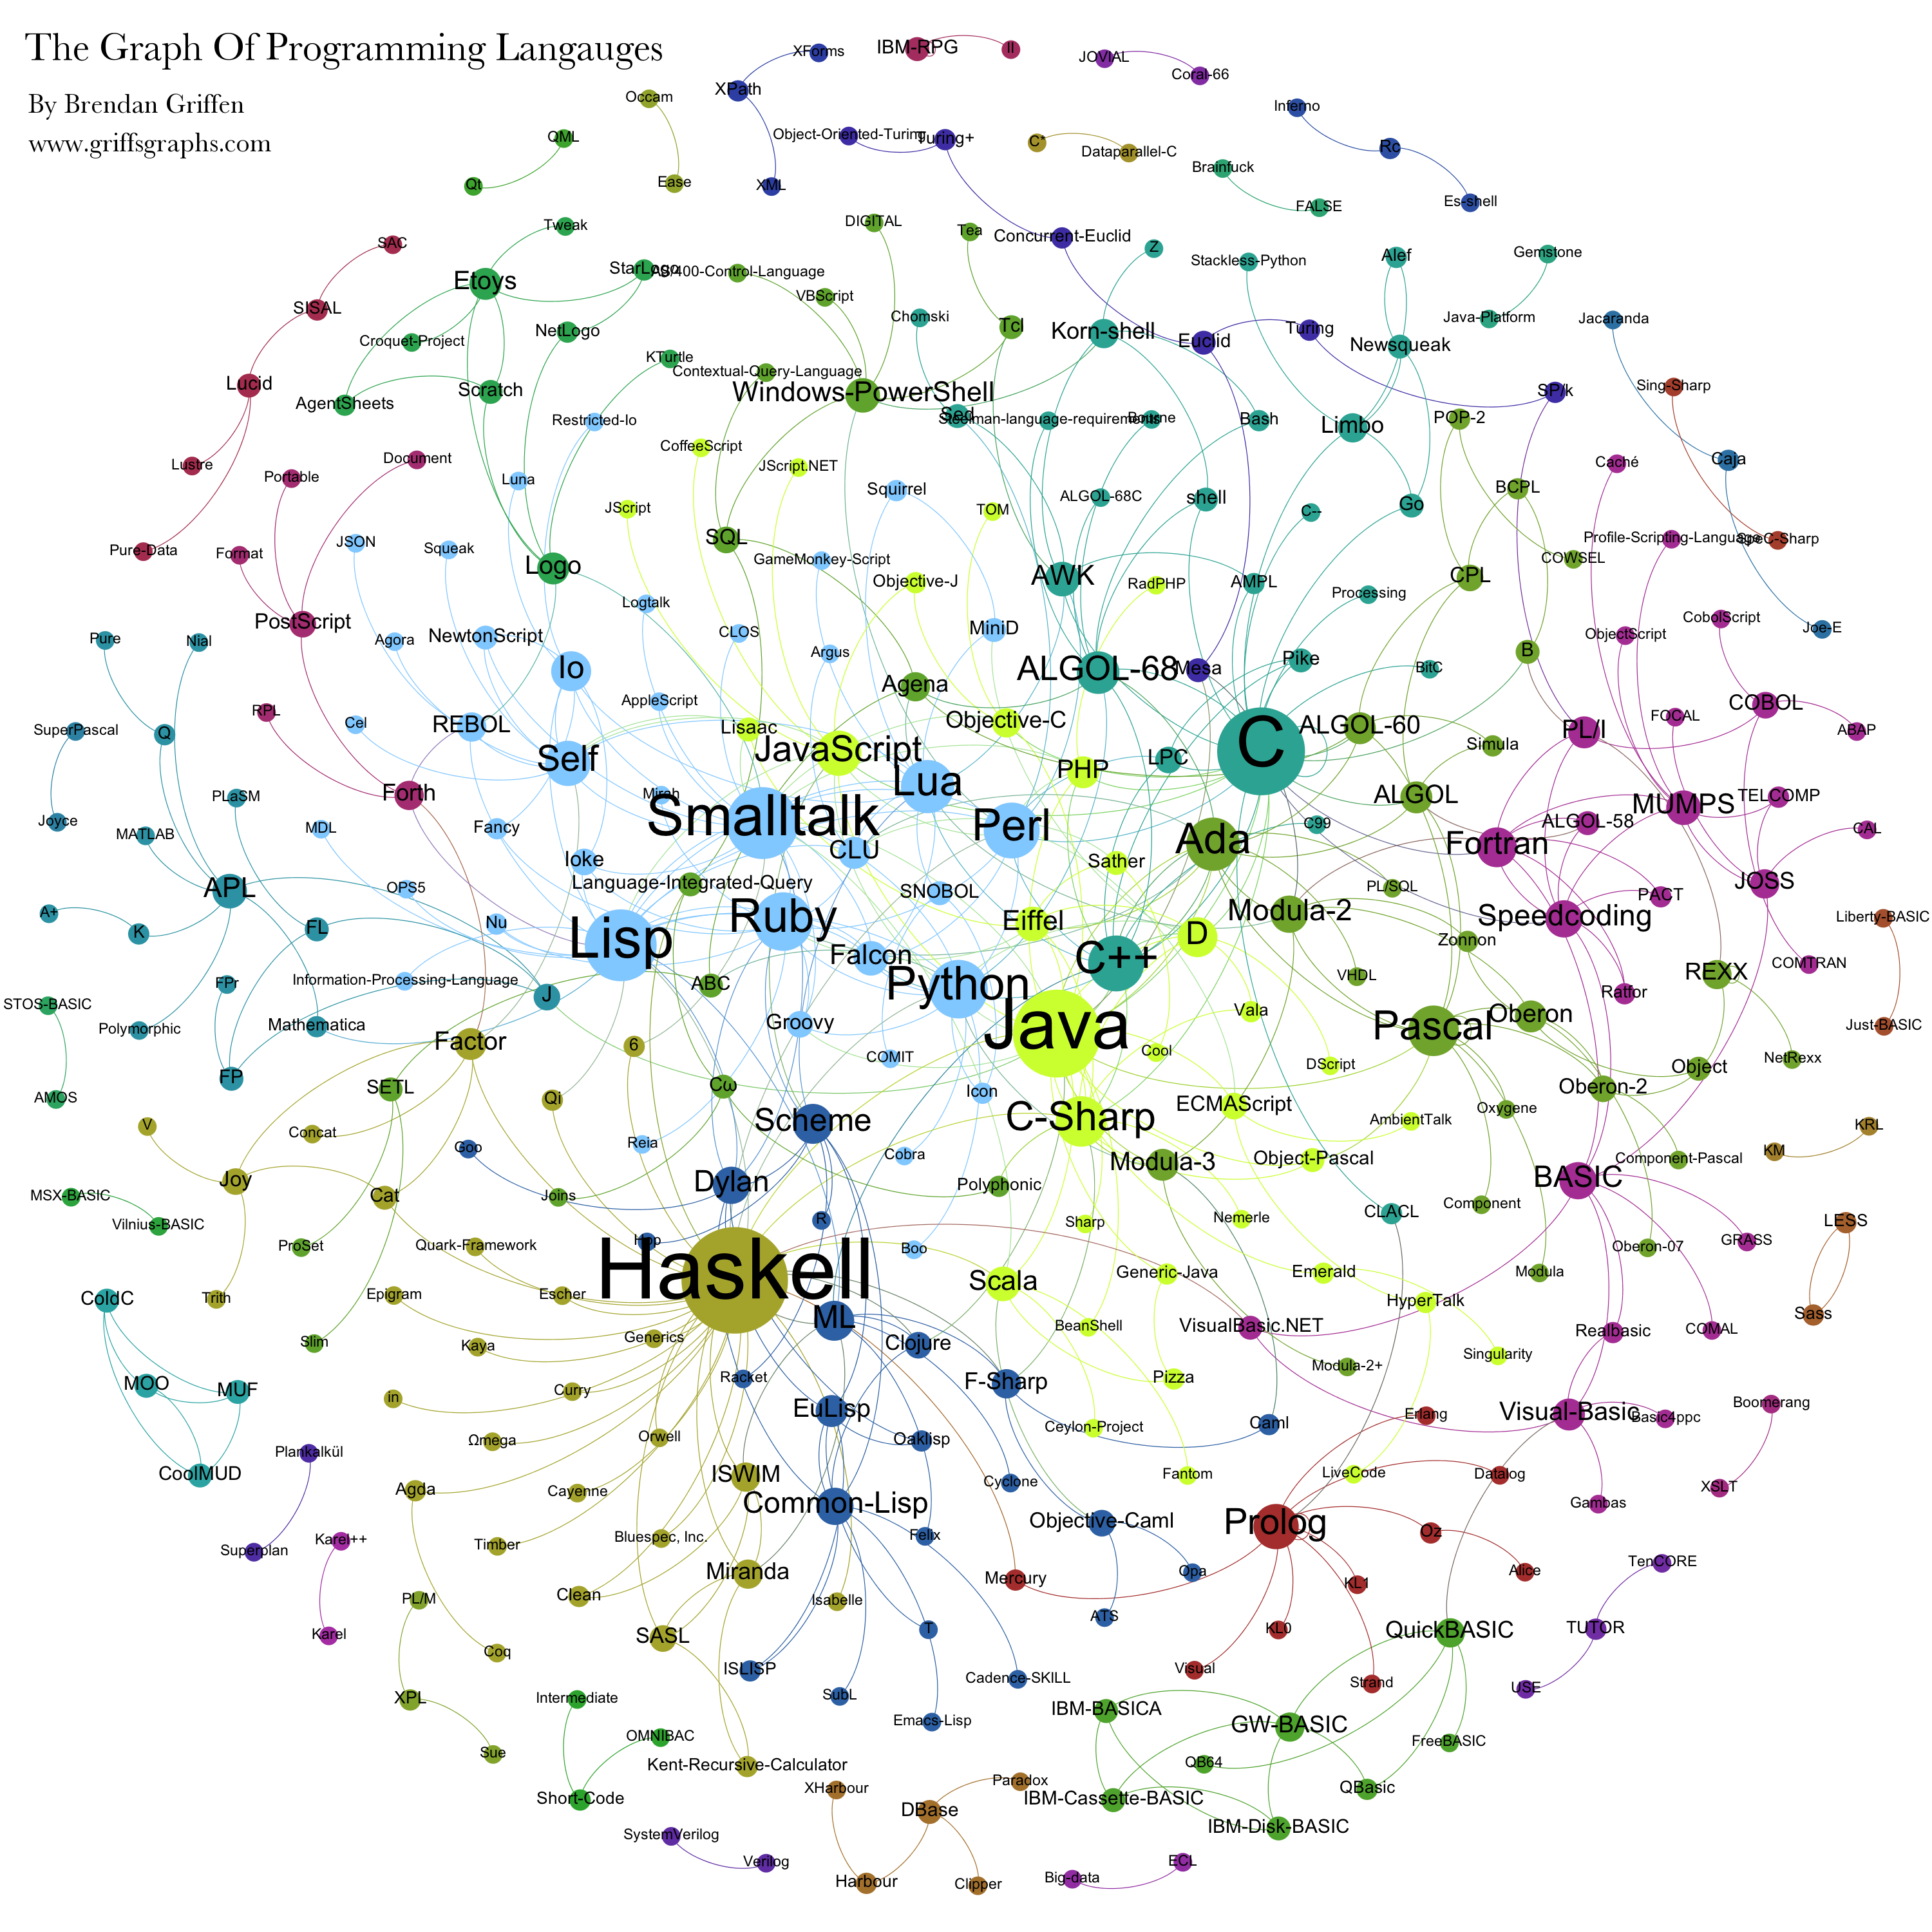
\includegraphics[height = 0.5\textwidth, width=0.5\textwidth]{programming-languages_2.png} 
    \caption{The Graph of programming Languages}
 \end{figure} 
 \note[item]{The graph depicts the varoius languages and how they are influenced and/or related to each other.}
\end{frame}

%% ====================================================================-
\subsection{Problem Statement}
\begin{frame}
   \frametitle{Thesis Statement}
   \begin{block}{Thesis statement}
     The thesis aims to provide insights into merging two declarative
     languages namely, \progLang{Haskell} and \progLang{Prolog} by
     embedding the latter into the former and analyzing the result of
     doing so\dots\,.
     \note[item]{\textcolor{red}{Read out Thesis statement.}}
   \end{block}
        \begin{itemize}
      \item Replicating functionality.
      \note[item]{One option is to replicate the target language funcitonality in the current environment,}
      
      \item \progLang{Prolog}-like functionality in \progLang{Haskell}.
      \note[item]{, and that is what we will look at today. Replicating \progLang{Prolog}-like functionality in \progLang{Haskell}}
      
      \item \textit{haskellised} \progLang{Prolog}-like eDSL
      \note[item]{The result is something close to a \textit{haskellised} \progLang{Prolog}, a functional eDSL with logic programming 
         capabilities.}
   \end{itemize}
\end{frame}

%% ====================================================================-
%% ====================================================================-
\section{Additional Concepts}
%% -------------------------------------------------------------------
\subsection{Monads}
\begin{frame}
	\frametitle{Monads}
\begin{itemize}
\item Monads in \progLang{Haskell} can be thought of as composable computation descriptions. They,
\note[item]{Monads are composable computation builders.}
\begin{itemize}
\item separate composition and computation execution time line,
\note[item]{separate how computations are composed and how they will be executed.}

\item carry and pass around data(state).
\note[item]{they hold results of the computation.}
\end{itemize}
\note[item]{This allows us to manipulat the control flow.}

\note[item]{This lends monads to supplementing pure calculations with features like I/O, common environment or state, etc.}

\item A monad is a structure that represents computations defined as sequences of steps.
\note[item]{Computations are a sequence of steps chained together.}

\item The monadic bubble.
\note[item]{Computations that produce side effects are carried out in a monad, a bubble, which prevents the outer state to get affected 
and hence the computation remains.}

\end{itemize}

\end{frame}
%% -------------------------------------------------------------------
	
%% -------------------------------------------------------------------
\subsection{Pattern Matching}
\begin{frame}[fragile]

\frametitle{Pattern Matching}
\begin{itemize}
\item In pattern matching, we attempt to match values against patterns and, if so desired, bind variables to successful matches.
\note[item]{In pattern matching, we matry and match values against patterns to bind values to variables.}
\note[item]{Pattern matching can either fail, succeed or diverge.}

\item Consider the example of the fibonacci series in \progLang{Haskell}.
\begin{minted}[linenos]{haskell}
fib 0 = 0
fib 1 = 1
fib n = fib (n-1) + fib (n-2)
\end{minted}
\note[item]{\progLang{Haskell} selects the appropriate computation depending on the result of matching the value of n to the patterns one by one.}

\end{itemize}

\end{frame}
%% -------------------------------------------------------------------

%% -------------------------------------------------------------------
\subsection{Unification}
\begin{frame}[fragile]
\frametitle{Unification}
\begin{itemize}
\item The way in which \progLang{Prolog} matches two terms is called unification. 
\note[item]{The idea is similar to that of unification in logic: we have two terms and we want to see if they can be made to represent the same structure.}
\begin{itemize}
\item If term1 and term2 are constants, then term1 and term2 unify if and only if they are the same atom, or the same number.
\note[item]{Constants are unified if they are the same.}
\item If term1 is a variable and term2 is any type of term, then term1 and term2 unify, and term1 is instantiated to term2 . Similarly, if term2 is a variable and term1 is any type of term, then term1 and term2 unify, and term2 is instantiated to term1 . (So if they are both variables, they’re both instantiated to each other, and we say that they share values.)
\note[item]{If one of the terms is a variable then it is instantiated to the other term.}

\item If term1 and term2 are complex terms, then they unify if and only if:
They have the same functor and arity, and
all their corresponding arguments unify, and
the variable instantiations are compatible.
\note[item]{For nested terms, we match the heads and the number of arguments before finding a unifier.}

\item Two terms unify if and only if it follows from the previous three clauses that they unify.
\end{itemize}
\end{itemize}
\end{frame}

%% -------------------------------------------------------------------
\begin{frame}[fragile] 
\frametitle{Unification Examples} 
\note[item]{Let us take a look at a few examples,}
\begin{itemize}
\item Unifying varaibles,

\begin{minted}[linenos]{prolog} 
(X,2) = (1,Y). 
X = 1. 
Y = 2.  
\end{minted}
\note[item]{In the first example, \prologConstruct{X} is instantiated to 1 and \prologConstruct{Y} to 2.}

\item  Unifying complex terms,

\begin{minted}[linenos]{prolog} 
k(s(g),Y) = k(X,t(k)). 
X = s(g) 
Y = t(k) 
\end{minted} 
\note[item]{The first check is to match the head of the two terms \prologConstruct{k}, next the arity and finally \prologConstruct{X} and
\prologConstruct{Y} are instantiated.}

\end{itemize}
	
\end{frame} 

%% ====================================================================-

\begin{comment}
\subsection{Motivation}
\begin{frame}{Motivation}
\frametitle{(to be discarded ......)}
\begin{itemize}
\item Language classification.
\note[item]{Languages are classified into categories known paradigms depending on their characteristics.}
\note[item]{Languages from the same paradigm may exhibit different properties.} 

\item For example, \progLang{Haskell}(functional language) and \progLang{Prolog}(logic language).
\note[item]{\progLang{Haskell} is a functional programming language while \progLang{Prolog} is a logic programming language.}
\note[item]{Both of them are declarative in nature but work differently.}

\item Scope.
\note[item]{The versatility of a programming language is how well it can adapt to a particular problem.}
\note[item]{For instance, \progLang{Prolog} is good for rule based systems. "Clarissa", a voice user interface for browsing space station procedures is written in SICStus
	Prolog[https://ti.arc.nasa.gov/m/pub-archive/999h/0999\%20\%28Rayner\%29.pdf].}
\end{itemize}
\end{frame}
\end{comment}





%% ====================================================================-
\begin{comment}
\subsection{Discarded Scope}
\begin{frame}{Scope}
\frametitle{(to be discarded ......)}
\begin{itemize}
\item General purpose programming languages.
\note[item]{A truly general purpose programming language, GPL, is described which contains facilities for constructing (within the 
language) new data types as well as facilities for operations performed upon them.[Jan V. Garwick. 1968. Programming Languages: GPL, a 
truly general purpose language. Commun. ACM 11, 9 (September 1968), 634-638. DOI=http://dx.doi.org/10.1145/364063.364092]} 

\item Domain specific programming languages.
\note[item]{A domain specific language is a concise micro language that offers tools and functionalities focused on solving problems ona  
particular domain.} 
\end{itemize}
\end{frame}
\end{comment}

%% ====================================================================-
%% ====================================================================-
\section{What was done}

\begin{frame}
\frametitle{Previously Existing Work}
\note[item]{Here we will look at the existing work,}
\begin{itemize}
\item Implementations.
\note[item]{Few exist. Incomplete and lack pratical features.}
\begin{itemize}
\item \codeLibrary{Mini Prolog} : \progLang{Prolog}-interpreter with support for variable search strategies.
\note[item]{micro \progLang{Prolog}-like language consisting only of atoms and variables. The interpreter can work with multiple strategies predetermined at compile time.}

\item \codeLibrary{prolog} : A \progLang{Prolog} interpreter written in \progLang{Haskell}.
\note[item]{is a more complete implementation consusting of \prologConstruct{cuts} and \prologConstruct{fails}.}

\item \progLang{Curry} : A functional logic programming based on \progLang{Haskell}
\note[item]{Works on the principles of residuation and narrowing to unify terms.}
\end{itemize}

\item Literature.
\note[item]{The literature mainly focuses on,}
\begin{itemize}
\item Translating \progLang{Prolog} predicates into a \progLang{Haskell} function.
\note[item]{A series of papers provide useful insights into replicating \progLang{Prolog}-like clauses in \progLang{Haskell} though none
	have accompanying implementations.}

\item Passing state of a computation.
\note[item]{state of each step in computation is passed on as a stream of answer substitutions,}

\item Implementing a typed functional logic programming language.
\note[item]{T6o get full static typing we need to use the \progLang{Haskell} extensions of quantified types and the \haskellConstruct{ST Monad}.}
\end{itemize}

\item Libraries.
\begin{itemize}
\item \codeLibrary{unification-fd} : Generic unification algorithms. 
\note[item]{generic unification algorithms which are imperative in nature.}

\item \codeLibrary{logict} : A continuation-based, backtracking, logic programming monad.
\note[item]{which allows us to add backtracking computations to any Haskell monad}

\end{itemize}

\end{itemize}

\end{frame}



%% ====================================================================-
%% ====================================================================-
\section{What we did}

%% -------------------------------------------------------------------
\begin{frame}{What we did Overview}
	
	\frametitle{What we did Overview}
\begin{itemize}
\item Literature review
  \begin{itemize}
  \item We reviewed literature on embedded languages (Chapter~5)
  \item We reviewed literature on merging programming
    languages (Chapter~6)
  \end{itemize}
\item Improvements,
\begin{itemize}
        \item Practical features.
	\note[item]{Firstly, we added practical features a \progLang{Prolog} distribution might, these being \prologConstruct{cut} and
		\prologConstruct{fail}.}
	
	\item \progLang{Prolog} in \progLang{Haskell}.
	\note[item]{Meaning, one can write a program in our eDSl just like one would write a \progLang{Haskell} program.}
\end{itemize}

\item Other Contributions,
\note[item]{In this section we will talk about, the contributions which are not neccessary an improvement on the current work but a new
	direction for solving the problem of embedding languages.}
\begin{itemize}
	\item Modular \textit{functorizing} mechanism.
	\note[item]{We open up the language to accomodate meta syntactic variables, custom quantifiers and logic.}
	
	\item Modular \textit{monadic} unification procedure.
	\note[item]{this is to leverage imperative unification algorithms.}
	
	\item Basic working \progLang{Prolog} implementation.
	\note[item]{}
	
	\item Variable search strategies.
	\note[item]{Independent of how the solution search happens our implementation must work.}
	
	\item Embedding IO in an eDSL. 
	\note[item]{Modularizing the interpreter in a manner so that each stage must only deal with a particular aspect of the program.}
	
\end{itemize}
\
\end{itemize}

\end{frame}
%% -------------------------------------------------------------------


%% ====================================================================-
\begin{comment}
	\subsection{Improvements}
\begin{frame}{Improvements}
\note[item]{The improvements,}
\begin{itemize}
\item Practical features.
\note[item]{Firstly, we added practical features a \progLang{Prolog} distribution might, these being \prologConstruct{cut} and
\prologConstruct{fail}.}

\item \progLang{Prolog} in \progLang{Haskell}.
\note[item]{Meaning, one can write a program in our eDSl just like one would write a \progLang{Haskell} program.}
\end{itemize}
\end{frame}

\end{comment}

%% ====================================================================-
\begin{comment}
	\subsection{Other Contributions}
\begin{frame}{Other Contributions}
\note[item]{In this section we will talk about, the contributions which are not neccessary an improvement on the current work but a new
direction for solving the problem of embedding languages.}
\begin{itemize}
\item Modular \textit{functorizing} mechanism.
\note[item]{We open up the language to accomodate meta syntactic variables, custom quantifiers and logic.}

\item Modular \textit{monadic} unification procedure.
\note[item]{this is to leverage imperative unification algorithms.}

\item Basic working \progLang{Prolog} implementation.
\note[item]{}

\item Variable search strategies.
\note[item]{Independent of how the solution search happens our implementation must work.}

\item Embedding IO in an eDSL. 
\note[item]{Modularizing the interpreter in a manner so that each stage must only deal with a particular aspect of the program.}

\end{itemize}
\end{frame}

\end{comment}

%% ====================================================================-
\subsection{Prototype 1}

\begin{frame}[fragile=singleslide]
	\frametitle{{Functorizing a language}}
	\begin{itemize}
		\item Consider the following recursive grammar,
		
		
		$1.  S \rightarrow aSb$
		
		
		$2. S \rightarrow ba$
		
		Example term : $ S \Rightarrow aSb \Rightarrow aaSbb \Rightarrow aababb $
		
		\note[item]{A recursive grammar locks you into the language and does not allow you introduce external ??quantifiers and logic??}
		
		\item Closed language,
		
		\begin{minted}[linenos]{haskell}
		data Term = Struct Atom [Term]
		| Var VariableName
		| Wildcard
		| Cut Int deriving (Eq, Data, Typeable)
		\end{minted}
		\note[item]{Our expressions can only be  built using \progLang{Term} and nothing else.}
		
		\item Open language,
		\begin{minted}[linenos]{haskell}
		data FlatTerm a = Struct Atom [a]
		|  Var VariableName
		|  Wildcard
		|  Cut Int deriving (Show, Eq, Ord)
		\end{minted}
		\note[item]{On the other hand, due to the addition of the type variable \haskellConstruct{a}, functionality can be injected into the language. }
		
	\end{itemize}
	
\end{frame}

\begin{frame}[fragile=singleslide]
	\frametitle{{Functorizing a language}}
	\begin{itemize}
		
		\item Manual extension,
		\begin{minted}[linenos]{haskell}
		data Term = Struct Atom [Term]
		| Var VariableName
		| Wildcard
		| Cut Int
		| New_Constructor_1 .........
		| New_Constructor_2 ......... 
		deriving (Eq, Data, Typeable, .....)
		\end{minted}
		\note[item]{A manual extension would result in modying the base language and the operations related to it.}
		
		\item Functorized Extension,
		\begin{minted}[linenos]{haskell}
		data Extended f = New_Constructor_1 ...
		| New_Constructor_2 ....
		| Base (f (Extended f)) 
		deriving (Eq, Data, Typeable, .....)
		\end{minted}
		\note[item]{Meanwhile, for the open language, a quantifier such as \haskellConstruct{Extended} can be used. }
	\end{itemize}
\end{frame}

\begin{frame}
	\frametitle{Monadic Unification}
	\note[item]{Here, we make use of the \codeLibrary{unification-fd} library }
	\begin{itemize}
		\item \codeLibrary{unification-fd} compatible
		\note[item]{Here, we make use of the \codeLibrary{unification-fd} library for providing the generic unification algorithm.}
		
		\item \textit{Unifiable} language.
		\note[item]{We create the necessary instances and make our language unifiable.}
		
		\item Convert the language expressions,    
		\note[item]{Convert the terms into \haskellConstruct{UTerm}}
		
		\item Extract and convert variables to become \haskellConstruct{State} compatible,
		\note[item]{the language varaibles are comnverted to state varaibles which store, pass and mutate values.}
		
		\item Carry out unification in the \haskellConstruct{Binding Monad}.
		\note[item]{The variables are bound to values representing substituions}
		
		\item Re translate substitutions.
		\note[item]{Extract state from the monad and translate the substitutions to the original language.}
	\end{itemize}
	
\end{frame}

\begin{frame}{Prototype 1}
\begin{figure}[H]
  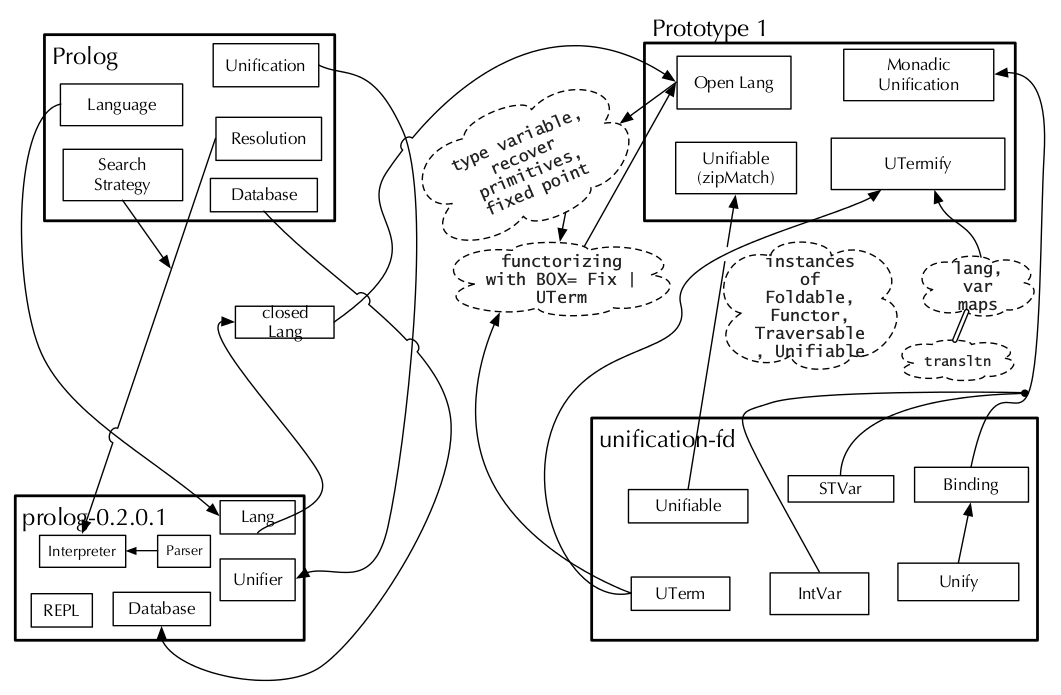
\includegraphics[width=1\textwidth, height=0.8\textheight]{Prototype-1-architecture.jpeg}
  \caption{Architecture of Prototype 1}
  \label{fig:proto1-arch}
\end{figure}
\note[item]{Let us take a look at the architecture for Prototype 1.}
\note[item]{We adopt a sample \progLang{Prolog}-like language}
\note[item]{The language is open up by introdcing a type variable.}
\note[item]{Make the language unifiable.}
\note[item]{Perform the unification in the monad.}
\note[item]{State is used to extract the substituion and return the result.}
\end{frame}


%% ====================================================================-
\subsection{Prototype 2}

\begin{frame}
\frametitle{Contributions}
\note[item]{For a logic programming language,}
\begin{itemize}
\item A query resolver matches a query to the rules in the knowledge base and generate a list of goals which when achieved a result is returned.
\note[item]{A query resolver matches a query to the rules in the knowledge base and generate a list of goals which when achieved a result is returned.}

\item A query resolver consists of,
\begin{itemize}
\item a scheduling policy,
\note[item]{ defines how the additions and deletions of goals from the resolvent is performed by the interpreter.}

\item a search strategy,
\note[item]{selecting possible alternatives while searching through a solution space.}

\item unification.
\note[item]{unify the terms in question to obtain a result.}
\end{itemize}  

\item Prototype 1 is only unification.
\note[item]{Prototype 1 is only unification.}

\item Prototype 2 is a \progLang{Prolog}-like interpreter.
\note[item]{The base implementation is taken from an already existing library for \progLang{Prolog} in \progLang{Haskell} and modified to accomodate an open grammar for the language and monadic unification.}
\note[item]{This prototype serves as a test to prove the modularity and flexibility of the procedures from prototype 1.}

\end{itemize}
\end{frame}

\begin{frame}{Prototype 2}
\begin{figure}[H]
  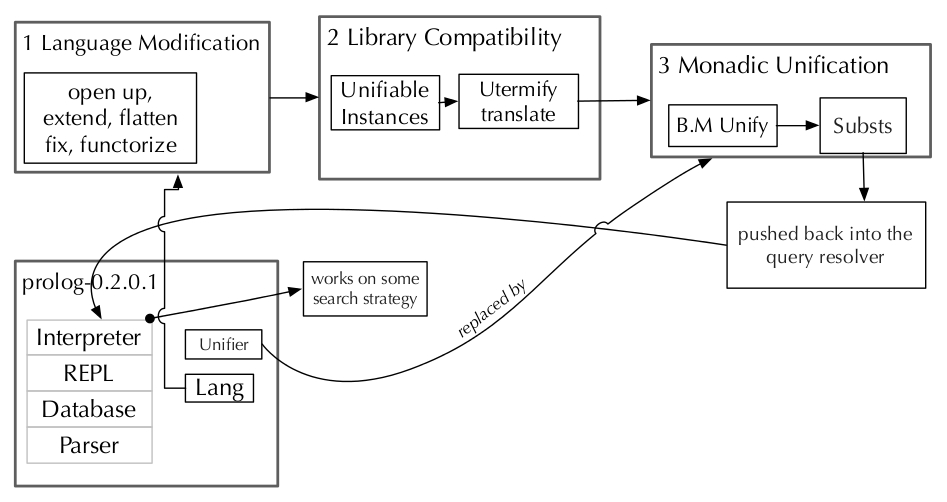
\includegraphics[width=1\textwidth, height=0.75\textheight]{Prototype-2-architecture.jpeg}
  \caption{Architecture of Prototype 2}
  \label{fig:proto1-arch}
\end{figure}
\note[item]{The procedure remain quite similar.}
\note[item]{Open up the language.}
\note[item]{Make it unifiable.}
\note[item]{Carry out the unification procedure.}
\note[item]{Extract and reconvert the results.}
\note[item]{Since this process takes place within the interpreter, the results are pushed back and the process continues.}
\end{frame}


%% ====================================================================-
\subsection{Prototype 3}

\begin{frame}
\frametitle{Contributions}
\note[item]{Prototype 2 demonstrated how the procedure can be applied to recursive grammars and carry out unification irrespective of the scheduling policy of the interpreter.}
\begin{itemize}
\item Variable search strategy,
\note[item]{In Prototype 3 we work with variable search strategies.}
\note[item]{The base implementation is based on a \progLang{Prolog}-like interpreter for \progLang{Haskell 98}.}

\note[item]{We work with 3 different search strategies,}
\begin{itemize}
\item Stack Engine,

\item Pure Engine, and,

\item Andorra Engine.
\end{itemize}

\end{itemize}
\end{frame}

\begin{frame}{Prototype 3}
\begin{figure}[H]
  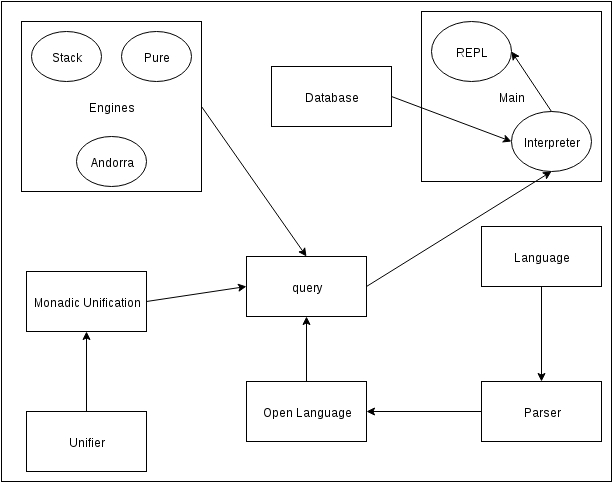
\includegraphics[width=0.75\textwidth, height=0.75\textheight]{Prototype-3-architecture.jpeg}
  \caption{Architecture of Prototype 3}
  \label{fig:proto1-arch}
\end{figure}
\note[item]{The procedure for Prototype 3 remains the same.}
\note[item]{The query resolver takes an additional input which is the search strategy at compile time.}
\end{frame}


%% ====================================================================-
\subsection{Prototype 4}

\begin{frame}
\frametitle{Contributions}

\begin{itemize}
\item Embedding input-output capabilities to a domain specific language.
\note[item]{Here we focus on embedding IO.}

\item Constructors for IO operations in the abstract syntax.
\note[item]{By defining constructors for IO operations in the language itself.}
\note[item]{one reason why this can be done is that funcitons in \progLang{Haskell} are first class citizens; they are data.}

\item Interpreted program is pure.
\note[item]{upon interpretation the program is still pure as no actions has been executed.}

\item Two-stage interpretation strategy.
\note[item]{Because of this we can have a two stage interpretation strategy.}
\end{itemize}
\end{frame}


\begin{frame}{Prototype 4}
\begin{figure}[H]
  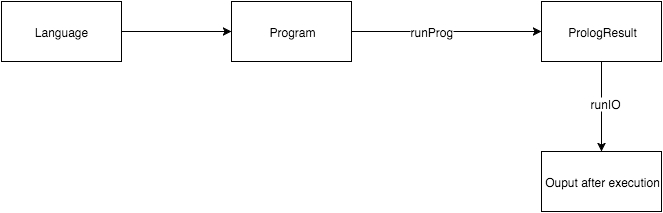
\includegraphics[width=1\textwidth]{Prototype-4-architecture.jpeg}
  \caption{Architecture of Prototype 4}
  \label{fig:proto1-arch}
\end{figure}
\note[item]{Consider Protoype 4.}
\note[item]{A program is written in a DSL is interpreted into a Result data type }
\note[item]{This consists of IO operations as constructors.}
\note[item]{The result is then run in the IO Monad(stage 2) producing the desired effects.}
\note[item]{So if the program does not consist of any IO operations the procedure remains pure through out.}
\note[item]{If it does, no problem the execution takes place in a monad anyways.}
\end{frame}


%% ====================================================================-
%% ====================================================================-
\section{What remains to be done}

\begin{frame}{Future Scope}
\begin{itemize}
\item Quasi quoter with antiquotation.
\note[item]{Quasiquoting allows programmers to use custom, domain-specific syntax to construct fragments of their program.} 
\note[item]{Antiquotation allows interchangeable usage of programming constructs of different languages in the same expression.}

\item Variable run time search strategy.
\note[item]{Currently prorotype 3 works with multiple search strategies but they need to specified at compile time. An addition would be enable the selection at run time.}

\item Additional database capabilities similar to \progLang{SWI Prolog}.
\note[item]{SWI \progLang{Prolog}, a popular \progLang{Prolog} distribution different database mechanisms.}
\begin{itemize}
\item \prologConstruct{assert/retract} database manipulation.
\note[item]{}

\item recorded database.
\note[item]{database terms are associated with a key}
\end{itemize}

\item Multi type variable language.
\note[item]{Currently the prototypes work with grammars with a single type. A multi type variable language would allow its contructotrs 
to be of different types.}

\item Prototype 4 additions and extension.
\note[item]{Additions and extension could be made to in the form of a hybrid constructor representing pure and impure operations.}
\end{itemize}

\end{frame}

%% ====================================================================-
%% ====================================================================-
\section{Conclusion}
%% ---------------------------------------------------------------------
\begin{frame}{Conclusion}
\note[item]{In conclusion, we set out to explore the various approaches for bringing languages together}
\begin{itemize}
\item Embedded domain specific language in \progLang{Haskell}.
\note[item]{support for eDSL's \progLang{Haskell}}

\item \progLang{Prolog}-like language which is closer to a \progLang{Prolog} distribution.
\note[item]{A more "complete" \progLang{Prolog} in \progLang{Haskell}.}

\item Prototype implementations.
\note[item]{We tested out methodologies for replicating functionalities with some prototypes.}

\item \progLang{Haskell}, an effective tool for embedding domain specific languages.
\note[item]{\progLang{Haskell}, an effective tool for embedding domain specific languages.}
\end{itemize}

\end{frame}
%% ---------------------------------------------------------------------

%% ---------------------------------------------------------------------
\begin{frame}{The End}
\begin{center}
\Huge Thank you!
\end{center}
\note[item]{That concludes the presentation.}
\note[item]{Ladies and gentlemen, thank you for your patience.}
\end{frame}
%% ---------------------------------------------------------------------

%% ---------------------------------------------------------------------
\begin{frame}{The End}
\begin{center}
\Huge Questions?
\end{center}
\note[item]{And questions please.}
\end{frame}
%% ---------------------------------------------------------------------

%% ---------------------------------------------------------------------
\begin{frame}
\Huge{\centerline{The End}}
\end{frame}
%% ---------------------------------------------------------------------

\begin{comment}
\section{Bibliography}
\begin{frame}[allowframebreaks]
	\frametitle{Bibliography}
	\setbeamertemplate{bibliography item}{[\theenumiv]}
	\nocite{*} 
	\bibliographystyle{plain} 
	\bibliography{Thesis-Presentation}
\end{frame}
\end{comment}

\clearpage



%----------------------------------------------------------------------------------------

\end{document} 
